\section{Evaluation}
\label{sec:eval}

\Mar{I think the high-level goal should be something along the lines
  of understanding prevalence of long test runs and main sources of
  cost in open-source Java projects.  Intuitively, the problem should
  come before the solution :).  Based on that, we study
  parallelization of testing frameworks.  More precisely, we
  investigage how prevalent test parallelization is, the potential for
  improving execution cost, issues of flakiness that hinders use of
  parallelization, and how to address those issues.}

We evaluated the characteristics of regression tests in open-source
development from a sample set of Java projects from
Github\Jbc{Remember to update the previous sentence after updating the
subject section}. We are interested in understanding the preva- lence
of long test runs, the main source of cost, and how often developers
explore parallelism to improve execution performance. We pose the
following research questions:

\newcommand{\RQA}{How prevalent is the occurence of time-consuming
regression tests in open-source projects?}
\newcommand{\RQB}{What is the distribution of CPU and IO bound
regression tests from the sample set?}
\newcommand{\RQC}{How the execution time is distributed among test
cases?}
\newcommand{\RQD}{How often developers use the parallelism features
from build manager systems to improve performance on test execution?}

\newcommand{\rqOne}{\textbf{RQ1.} \RQA}
\newcommand{\rqTwo}{\textbf{RQ2.} \RQC}
\newcommand{\rqThree}{\textbf{RQ3.} \RQB}
\newcommand{\rqFour}{\textbf{RQ4.} \RQD}

\begin{itemize}
    \item \rqOne
    \item \rqTwo
    \item \rqThree
    \item \rqFour
\end{itemize}

The first research question addresses the distribution of subjects per
elapsed time to execute regression tests. We are interested on
identifying time-consuming test suites for further investigation. The
second research question addresses the distribution of execution time
per test case for each project. The rationale is that if the time cost
of a regression test is equally distributed among test cases, the
execution cost could be potentially improved by running tests in
parallel (in contrast to the scenario where only one test case
dominates most of the execution time).

\subsection{Subjects}
\label{sec:subjects}

\Jbc{Subject selection is currently OK but I will use another way (eg
Google BigQuery) to have access to more subjects.}We used the Github's
Search API~\cite{githubsearch} to fetch the top 1,000\footnote{The
Search API imposes the limit of 1,000 results regardless of the number
of matches from a search criteria.} Java projects with at least 100
stars. The number of stars indicates the interest and appreciation
from the community to a given project.
\Comment{(https://help.github.com/articles/about-stars/)} Although our
criteria is subjective, it is an approximation to find relevant
projects to conduct our study. We detected the build manager system
based on the files located in the root directory from the project in
the following precedence: Maven (\emph{pom.xml)}, Gradle
(\emph{gradlew}), and Ant (\emph{build.xml}).\Jbc{Remember to update
the following values after updating the subject selection approach.}
From the 1,000 downloaded projects, we detected the build system of
801 subjects (composed by 216 Maven, 564 Gradle, and 21 Ant projects)
and considered 164 projects that we were able to compile (153 Maven
and 9 Ant projects).  We were unable to compile other subjects because
some are related to a particular platform (\eg, Gradle implied
Android), unsolved dependencies, or the build process is based on
user-defined tasks (\eg, we considered the name \emph{compile} on Ant
projects).

\subsection{Setup and Replication}
\label{sec:setup}

To run our experiments, we used a \emph{Core i7-4790} (3.60 GHz) Intel
processor machine with 8 virtual CPUs (4 cores with 2 native threads
each) and 16GB of memory, running \emph{Ubuntu 14.04 LTS Trusty Tahr}
(64-bit version). Software settings include the Linux \emph{sysstat}
package to measure performance, \emph{git} to fetch subjects,
\emph{Java 8} to build and test subjects, and \emph{Python 3.4} to run
our evaluation scripts. For replication, we provide all the source
artifacts publicly available at \Fix{create gh-pages}, including
supporting scripts (\eg, the script that test subjects and generates
the raw data), the full list of projects, and a \emph{Vagrantfile} to
emulate our hardware and all software dependencies properly configured.

\subsection{Answering research question RQ1}
\label{sec:rqone}

\begin{itemize}
    \item \RQA
\end{itemize}

To evaluate the frequency of time-consuming regression tests, we first
compiled source and test files, later, we measured the elapsed time to
run the tests via the build system ignoring non-related tasks (\eg,
\emph{javadoc} generation).  We grouped the subjects according to the
execution time: tests that ran in less than one minute (\emph{short
execution}), one to five minutes (\emph{medium execution}), and more
than five minutes (\emph{long execution}).
Figure~\ref{fig:piechart-time} shows the proportion of subjects per
group. It is important to mention that Figure~\ref{fig:piechart-time}
represents a lower bound for elapsed time: some tests may finish early
due to a failure since the subjects were tested in a potentially
unstable revision.

\begin{figure}[h!]
    \centering
    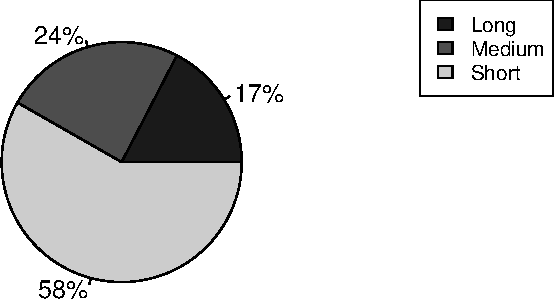
\includegraphics[width=0.4\textwidth]{results/rq1/plots/piechart.pdf}
    \caption{\label{fig:piechart-time} Subjects grouped by elapsed
    time on test execution ($t$): short execution ($t < 1m$), medium 
    execution ($1m \leq t < 5m$), and long execution ($5m \leq t$).}
\end{figure}

For the subjects from the groups \emph{medium} and \emph{long}, we
compared the execution time and the number of tests successfully
executed. As expected, Figure~\ref{fig:scatters} reveals that the
number of tests cases are not related to the elapsed time.
\Fix{explain briefly what dominates a test execution/types of tests}.
We ignored outliers for better visualization.

\begin{figure}[h!]%
    \centering
    \begin{minipage}{0.5\textwidth}
        \subfigure[\Fix{medium}]{
            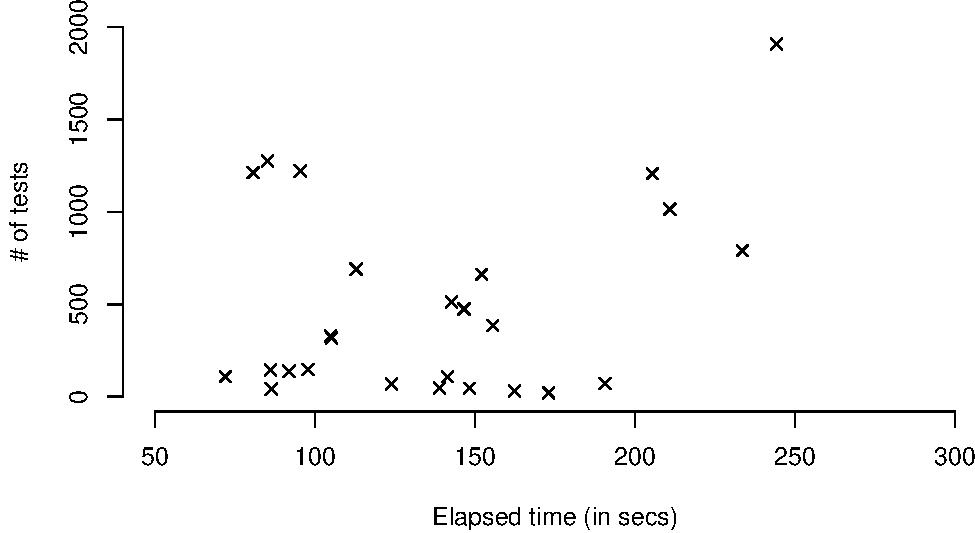
\includegraphics[width=\textwidth]{results/rq1/plots/scatterplot-med.pdf}
        }\\
        \subfigure[\Fix{long}]{
            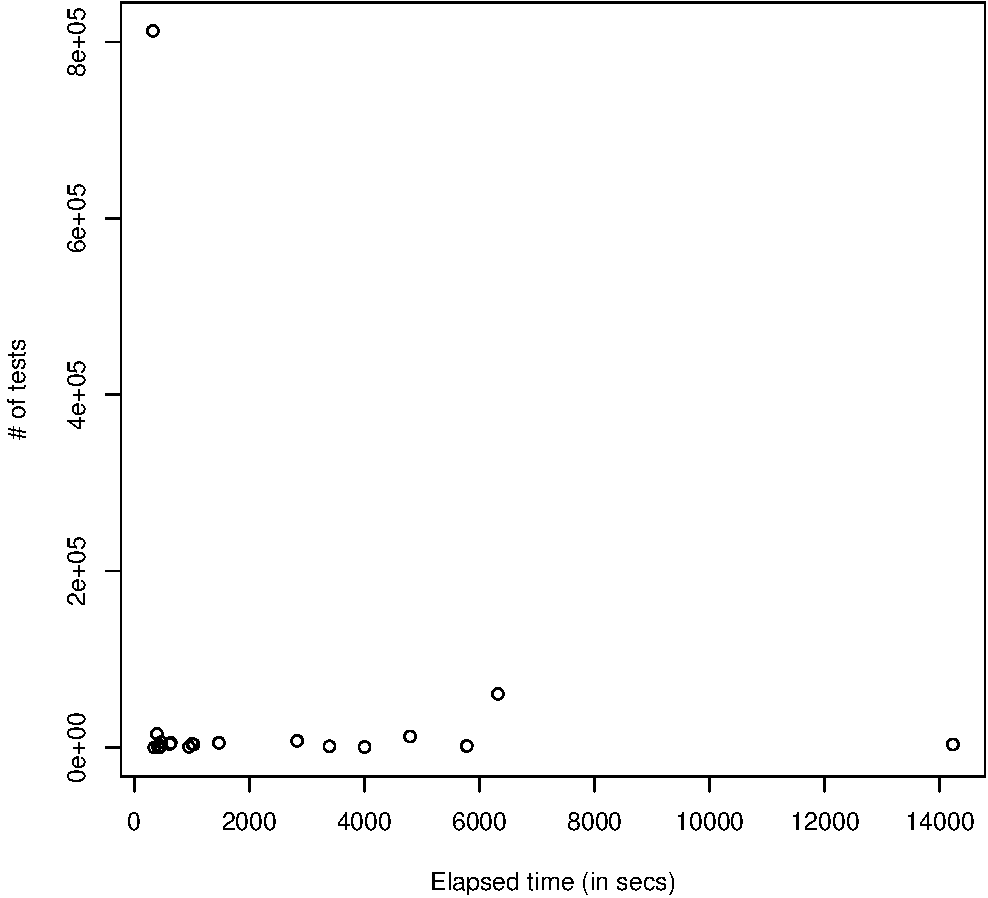
\includegraphics[width=\textwidth]{results/rq1/plots/scatterplot-long.pdf}
        }%
    \end{minipage}%
    \caption{\Fix{...use minutes instead of secs...}}%
    \label{fig:scatters}%
\end{figure}

\subsection{Answering research question RQ2}
\label{sec:rqTwo}

\begin{itemize}
    \item \RQC
\end{itemize}

To evaluate the distribution of execution time, we calculated the cost
from 90\% of test cases ordered by execution time and compared the
resulting value to the total time.  We collected the elapsed time from
test cases for each generated report. Maven Surefire generates an XML
report with execution information (\eg, number of skipped tests and
elapsed time) per test suite \Jbc{Should I use the previous sentence
as a footnote or should I delete it?}. We noticed that some test cases
reported an elapsed time of zero: since the reported time is in
milliseconds, some tests may execute in a shorter time. \Fix{..to be
continued...}

\begin{figure}[h!]
    \centering
    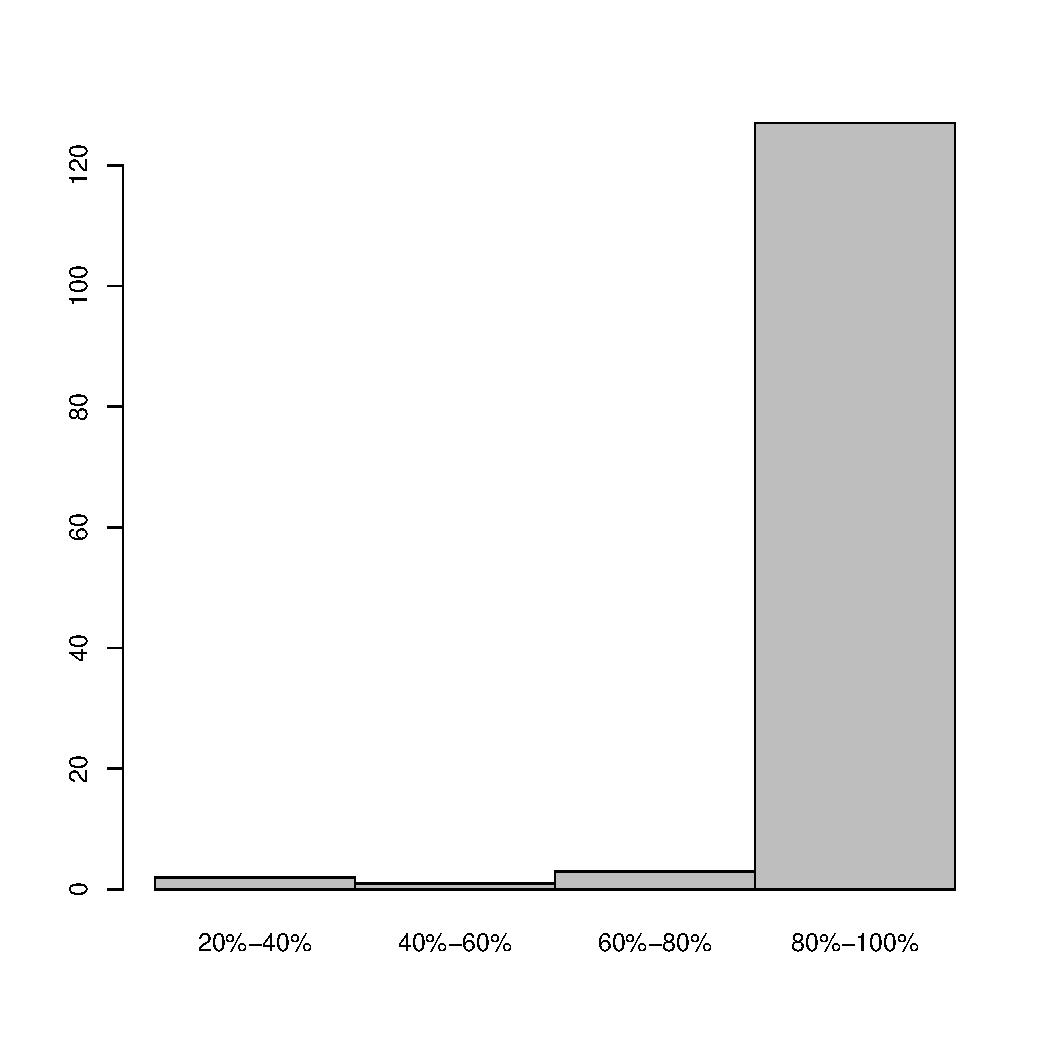
\includegraphics[width=0.4\textwidth]{figs/tcdistrib.pdf}
    \caption{\Fix{...}}
\end{figure}

\subsection{Answering research question RQ3}
\label{sec:rqThree}

\begin{itemize}
    \item \RQB
\end{itemize}

To evaluate the distribution of CPU and IO bound in regression tests
from the sample set, we proposed the definition of \emph{cpuness}
computed as the follow: $((user\_t + system\_t) / elapsed\_t) * 100$,
where \emph{user\_t} is the elapsed time of execution in \emph{user
mode}, \emph{system\_t} is the elapsed in \emph{kernel mode}, and
\emph{elapsed\_t} is the elapsed time to finish the execution. We
measured the \emph{cpuness} of each regression test \Fix{...elaborate
the meaning of cpuness} \Fix{Describe how I measured user, system and
"wall" time}.  \Fix{Explain results}.  \Fix{show plots}

\subsection{Answering research question RQ4}
\label{sec:rqfour}

%% \begin{itemize}
%%     \item \RQFOUR
%% \end{itemize}

\Fix{to appear...}

